\documentclass[12pt, a4paper]{report}
%\usepackage[a4paper]{geometry}

\usepackage{indentfirst}
%\setlengh{\parindent}{20pt}


\usepackage[spanish]{babel}
\usepackage{amsmath}
\usepackage{amssymb}
\usepackage{graphicx}
\usepackage{float}
\usepackage{titlesec}
\usepackage{paralist}
\usepackage{fancyvrb}
\usepackage[toc,page]{appendix}

% \usepackage{listings}
% \usepackage{xcolor}




\usepackage{xargs}                      % Use more than one optional parameter in a new commands
\usepackage[pdftex,dvipsnames]{xcolor}  % Coloured text etc.
\usepackage[colorinlistoftodos,prependcaption,textsize=small]{todonotes}
\usepackage{hyperref}
\usepackage{listings}
\usepackage[T1]{fontenc}
\usepackage{textcomp}
\newcommandx{\borrar}[2][1=]{\todo[linecolor=red,backgroundcolor=red!25,bordercolor=red,#1]{#2}}
\newcommandx{\corregir}[2][1=]{\todo[linecolor=blue,backgroundcolor=blue!25,bordercolor=blue,#1]{#2}}
\newcommandx{\info}[2][1=]{\todo[linecolor=OliveGreen,backgroundcolor=OliveGreen!25,bordercolor=OliveGreen,#1]{#2}}
\newcommandx{\pendiente}[2][1=]{\todo[linecolor=Plum,backgroundcolor=Plum!25,bordercolor=Plum,#1]{#2}}
\newcommandx{\thiswillnotshow}[2][1=]{\todo[disable,#1]{#2}}

\definecolor{codegreen}{rgb}{0,0.6,0}
\definecolor{codegray}{rgb}{0.5,0.5,0.5}
\definecolor{codepurple}{rgb}{0.58,0,0.82}
\definecolor{backcolour}{rgb}{0.95,0.95,0.92}
\lstdefinestyle{mystyle}{
    backgroundcolor=\color{backcolour},
    commentstyle=\color{codegreen},
    keywordstyle=\color{magenta},
    numberstyle=\tiny\color{codegray},
    stringstyle=\color{codepurple},
    basicstyle=\ttfamily\footnotesize,
    breakatwhitespace=false,
    breaklines=true,
    captionpos=b,
    keepspaces=true,
    numbers=left,
    numbersep=5pt,
    showspaces=false,
    showstringspaces=false,
    showtabs=false,
    tabsize=2,
	inputencoding=utf8, extendedchars=true, literate      =        % Support additional characters
      {á}{{\'a}}1  {é}{{\'e}}1  {í}{{\'i}}1 {ó}{{\'o}}1  {ú}{{\'u}}1
      {Á}{{\'A}}1  {É}{{\'E}}1  {Í}{{\'I}}1 {Ó}{{\'O}}1  {Ú}{{\'U}}1
      {à}{{\`a}}1  {è}{{\`e}}1  {ì}{{\`i}}1 {ò}{{\`o}}1  {ù}{{\`u}}1
      {À}{{\`A}}1  {È}{{\`E}}1  {Ì}{{\`I}}1 {Ò}{{\`O}}1  {Ù}{{\`U}}1
      {ä}{{\"a}}1  {ë}{{\"e}}1  {ï}{{\"i}}1 {ö}{{\"o}}1  {ü}{{\"u}}1
      {Ä}{{\"A}}1  {Ë}{{\"E}}1  {Ï}{{\"I}}1 {Ö}{{\"O}}1  {Ü}{{\"U}}1
      {â}{{\^a}}1  {ê}{{\^e}}1  {î}{{\^i}}1 {ô}{{\^o}}1  {û}{{\^u}}1
      {Â}{{\^A}}1  {Ê}{{\^E}}1  {Î}{{\^I}}1 {Ô}{{\^O}}1  {Û}{{\^U}}1
      {œ}{{\oe}}1  {Œ}{{\OE}}1  {æ}{{\ae}}1 {Æ}{{\AE}}1  {ß}{{\ss}}1
      {ẞ}{{\SS}}1  {ç}{{\c{c}}}1 {Ç}{{\c{C}}}1 {ø}{{\o}}1  {Ø}{{\O}}1
      {å}{{\aa}}1  {Å}{{\AA}}1  {ã}{{\~a}}1  {õ}{{\~o}}1 {Ã}{{\~A}}1
      {Õ}{{\~O}}1  {ñ}{{\~n}}1  {Ñ}{{\~N}}1  {¿}{{?`}}1  {¡}{{!`}}1
      {°}{{\textdegree}}1 {º}{{\textordmasculine}}1 {ª}{{\textordfeminine}}1
      {£}{{\pounds}}1  {©}{{\copyright}}1  {®}{{\textregistered}}1
      {«}{{\guillemotleft}}1  {»}{{\guillemotright}}1  {Ð}{{\DH}}1  {ð}{{\dh}}1
      {Ý}{{\'Y}}1    {ý}{{\'y}}1    {Þ}{{\TH}}1    {þ}{{\th}}1    {Ă}{{\u{A}}}1
      {ă}{{\u{a}}}1  {Ą}{{\k{A}}}1  {ą}{{\k{a}}}1  {Ć}{{\'C}}1    {ć}{{\'c}}1
      {Č}{{\v{C}}}1  {č}{{\v{c}}}1  {Ď}{{\v{D}}}1  {ď}{{\v{d}}}1  {Đ}{{\DJ}}1
      {đ}{{\dj}}1    {Ė}{{\.{E}}}1  {ė}{{\.{e}}}1  {Ę}{{\k{E}}}1  {ę}{{\k{e}}}1
      {Ě}{{\v{E}}}1  {ě}{{\v{e}}}1  {Ğ}{{\u{G}}}1  {ğ}{{\u{g}}}1  {Ĩ}{{\~I}}1
      {ĩ}{{\~\i}}1   {Į}{{\k{I}}}1  {į}{{\k{i}}}1  {İ}{{\.{I}}}1  {ı}{{\i}}1
      {Ĺ}{{\'L}}1    {ĺ}{{\'l}}1    {Ľ}{{\v{L}}}1  {ľ}{{\v{l}}}1  {Ł}{{\L{}}}1
      {ł}{{\l{}}}1   {Ń}{{\'N}}1    {ń}{{\'n}}1    {Ň}{{\v{N}}}1  {ň}{{\v{n}}}1
      {Ő}{{\H{O}}}1  {ő}{{\H{o}}}1  {Ŕ}{{\'{R}}}1  {ŕ}{{\'{r}}}1  {Ř}{{\v{R}}}1
      {ř}{{\v{r}}}1  {Ś}{{\'S}}1    {ś}{{\'s}}1    {Ş}{{\c{S}}}1  {ş}{{\c{s}}}1
      {Š}{{\v{S}}}1  {š}{{\v{s}}}1  {Ť}{{\v{T}}}1  {ť}{{\v{t}}}1  {Ũ}{{\~U}}1
      {ũ}{{\~u}}1    {Ū}{{\={U}}}1  {ū}{{\={u}}}1  {Ů}{{\r{U}}}1  {ů}{{\r{u}}}1
      {Ű}{{\H{U}}}1  {ű}{{\H{u}}}1  {Ų}{{\k{U}}}1  {ų}{{\k{u}}}1  {Ź}{{\'Z}}1
      {ź}{{\'z}}1    {Ż}{{\.Z}}1    {ż}{{\.z}}1    {Ž}{{\v{Z}}}1
      % ¿ and ¡ are not correctly displayed if inconsolata font is used
      % together with the lstlisting environment. Consider typing code in
      % external files and using \lstinputlisting to display them instead.}
}

\lstset{style=mystyle}

\title{Trabajo Práctico Final}
\author{Guillermo Rolle}

%\parindent 20pt

\begin{document}
	\begin{titlepage}
		\makeatletter
		\begin{center}
			\vspace{1cm}
			\Huge
			\textbf{\@title}

			\vspace{0.5cm}
			\LARGE
			Robótica Móvil

			\vspace{1.5cm}

			\textbf{Alumno: }\@author\\


			\vfill

			\Large
			Curso de Posgrado\\FCEIA-UNR

			\vspace{1.5cm}
			\textbf{Docente: }Taihú Pire

			\vspace{0.8cm}
			% \includegraphics[width=0.4\textwidth]{university}
			\Large
			\today
		\end{center}
		\makeatother
	\end{titlepage}

	\begin{abstract}

		En este trabajo se implementó un sistema de localización basado en visión por computadora para un manipulador móvil que debe desplazarse en un ambiente interior como, por ejemplo, una fábrica. Los algoritmos fueron implementados en ROS2 y son probados mediante simulación en Gazebo.

		El manipulador móvil utilizado es un prototipo de diseño que fue realizado para un Proyecto de Vinculación Tecnológica con una PyME metalúrgica local. Un problema típico que existe para este tipo de bases móviles es el problema de la localización, motivo por el cuál se eligió esta línea de trabajo, buscando resolver el problema de localización de una forma económica pero funcional.

		En este informe se desarrollará por completo el trabajo realizado, la idea conceptual, los detalles de implementación en ROS y de la simulación en Gazebo; y la configuración y scripts para ejecutar los distintos nodos para reproducir los resultados.
	\end{abstract}

	\newpage
	\tableofcontents
	\newpage

	\listoftodos[Lista de Pendientes]
	\newpage

    \chapter{Introducción}\label{ch:intro}
		\section{Motivación}\label{sec:motivacion}
			El trabajo desarrollado en el presente informe es una extensión de un Proyecto de Vinculación con el Medio, llevado a cabo por el LAC (Laboratorio de Automatización y Control) en conjunto con una PyME metalmecánica rosarina, enmarcado en el Programa TecnoPyME 2023 de la Provincia de Santa Fe.

			En dicho proyecto, se hizo un prediseño mecánico conceptual de un manipulador móvil que permitiría transportar insumos entre los distintos sectores y estaciones de trabajo dentro de la fábrica.
			La base móvil fue desarrollada pensando en la modularidad de la misma.
			Es decir, se diseñó un único chasis que permitiría dotarlo de diferentes estructuras de operación y sistemas locomoción, según los requisitos y necesidades del cliente.
			De esta forma, se busca disminuir los costos de fabricación y maximizar la cantidad de configuraciones posibles del manipulador móvil mediante el acople/desacople de distintos módulos.

			En cuanto a la localización de la base móvil dentro de la fábrica, a priorí, se pensó únicamente en procesar la información provista por la odometría de las ruedas motrices.
			Este método por sí sólo no permite una buena navegación dado que no hay ningún sensor exteroceptivo que procese información del entorno y la odometría acumula error rápidamente, tanto en presencia de deslizamiento de las ruedas, como por errores de parametrización.
			Por este motivo, en este trabajo se propone un método para mejorar la estimación la pose del robot utilizando visíón por computadora.

		\section{Repositorios}\label{sec:repositorios}
	El algoritmo de localización utilizando visión por computadora fue implementado en ROS2 y fue probado por simulación en Gazebo.
			Todos los archivos utilizados se encuentran en un repositorio de GitHub\footnote{\url{https://github.com/guillerolle/carrolac-project}}.

			En el mismo se encuentran las fuentes completas del workspace de ROS, incluyendo los archivos para la simulación en Gazebo; un archivo DockerFile con varios scripts de utilidad para ejecutar las simulaciones en el contenedor Docker; y los archivos fuentes de este mismo informe.

			Por otra parte, se creó un video demostrativo del funcionamiento del algoritmo en YouTube\footnote{\url{https://youtu.be/1lgu2i4TX7Q}}.
			En el video se muestra directamente la visualización en Rviz, comparando las trayectorias con y sin la corrección.

			Por último, para reproducir los resultados (o realizar modificaciones en el algoritmo) en otra computadora sin tener que ejecutar una simulación en Gazebo desde cero, se subió un archivo bag de ROS de un ensayo en particular en Mega\footnote{\url{https://mega.nz/file/q0R3BYCK#S2Pc1iaddbtkwS_2Mw9nvdmk7yq-gsmmCQf6HnYI-aI}} con todos los tópicos necesarios.

		\section{Manipulador Móvil}\label{sec:manipulador-movil}
			La base móvil utilizada es un prototipo conceptual desarrollado por el LAC para una PyME metalmecánica local, a la que se le adosó un manipulador \emph{Scorbot ER-IX} (existente en el LAC) para emular el comportamiento de manipulador móvil.
			Se hace notar que, a fines de este trabajo práctico final de la materia, no hay ningún tipo de control sobre el manipulador y sólamente se busca mejorar la localización de la base móvil.
			El manipulador adosado, en este contexto, puede ser considerado parte de la base móvil.

			En la Figura~\ref{fig:carrolac} se muestra la configuración del manipulador móvil en el entorno de Gazebo.
			El sistema de locomoción consta con un módulo de tracción diferencial atrás y dos ruedas cásters en el frente.
			El módulo con el manipulador, acoplado a la base móvil en parte trasera, tiene una rueda cáster también que hace de apoyo.
			En el frente, la base móvil tiene acoplado un módulo de sensores: éste tiene una cámara monocular, un sensor LiDaR 360° y una IMU.
			A los fines de este trabajo, el LiDaR sólamente se utiliza como visualización en Rviz y la IMU es ignorada completamente.
		
			\begin{figure}[H]
				\centering
				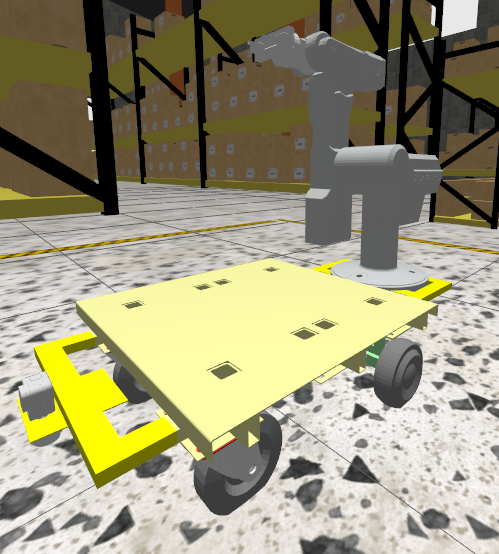
\includegraphics[width=0.7\linewidth]{img/CARROLAC}
				\caption[Carrolac]{Manipulador móvil en Gazebo}
				\label{fig:carrolac}
			\end{figure}

		\section{Marcadores ArUco}\label{sec:marcadores-aruco}
			Este método propone la utilización de marcadores ArUco\footnote{\url{https://docs.opencv.org/4.x/d5/dae/tutorial\_aruco\_detection.html}} para estimar la pose del robot.

			Los marcadores ArUco son marcadores cuadrados que están dotados de una matriz binaria blanca y negra que codifica el identificador único del marcador en su interior y tienen un borde negro que permite la rápida detección del mismo.
			A su vez, el tamaño del marcador determina el tamaño de la matriz interna.
			Por ejemplo, un marcador de tamaño 4x4 está compuesto por 16 bits.
			En la Figura~\ref{fig:markers} se muestran ejemplos de marcadores ArUco de distinto tamaño.

			\begin{figure}[H]
				\centering
				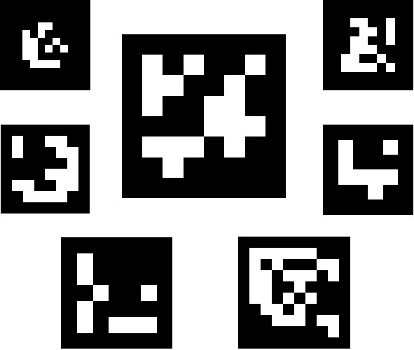
\includegraphics[width=0.7\linewidth]{img/markers}
				\caption[Carrolac]{Ejemplos de marcadores ArUco}
				\label{fig:markers}
			\end{figure}

			Los marcadores pueden ser encontrados girados en el entorno, por lo que el proceso detección debe permitir determinar su orientación original para que cada esquina sea identificada inequívocamente.
			Esto también se hace basándose en la codificación binaria.

			En este trabajo se utilizaron marcadores tamaño 6x6, con un diccionario de tamaño de 50 marcadores.
			En la Figura~\ref{fig:aruco} se muestran dos marcadores ArUco dispuestos en el entorno de simulación de Gazebo.
			\begin{figure}[H]
				\centering
				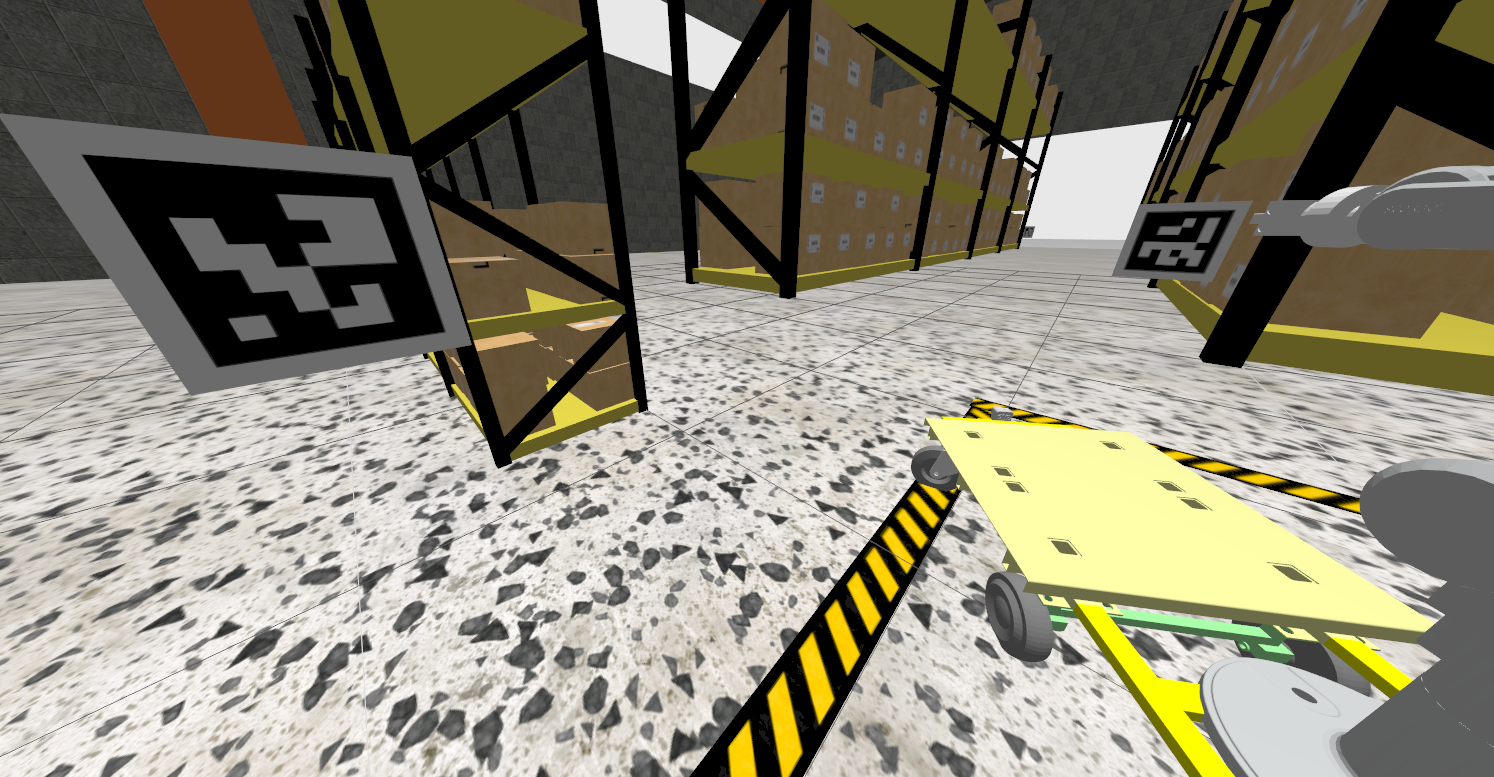
\includegraphics[width=0.9\linewidth]{img/aruco}
				\caption[Carrolac]{Marcadores ArUco en Gazebo}
				\label{fig:aruco}
			\end{figure}

	\chapter{Algoritmo de localización}\label{ch:algoritmo-localizacion}
		\section{Idea conceptual}\label{sec:algoritmo-localizacion/idea-conceptual}
			Conceptualmente, la idea es ubicar varios marcadores ArUco en posiciones y orientaciones conocidas dentro de la fábrica y utilizar la cámara para determinar la pose relativa entre el marcador y la base móvil.

			En la Figura~\ref{fig:cv_aruco} se muestra una captura de la cámara del robot, en donde se ven 2 marcadores ArUco con sus correspondientes sistemas de referencia locales detectados.
			\begin{figure}[H]
				\centering
				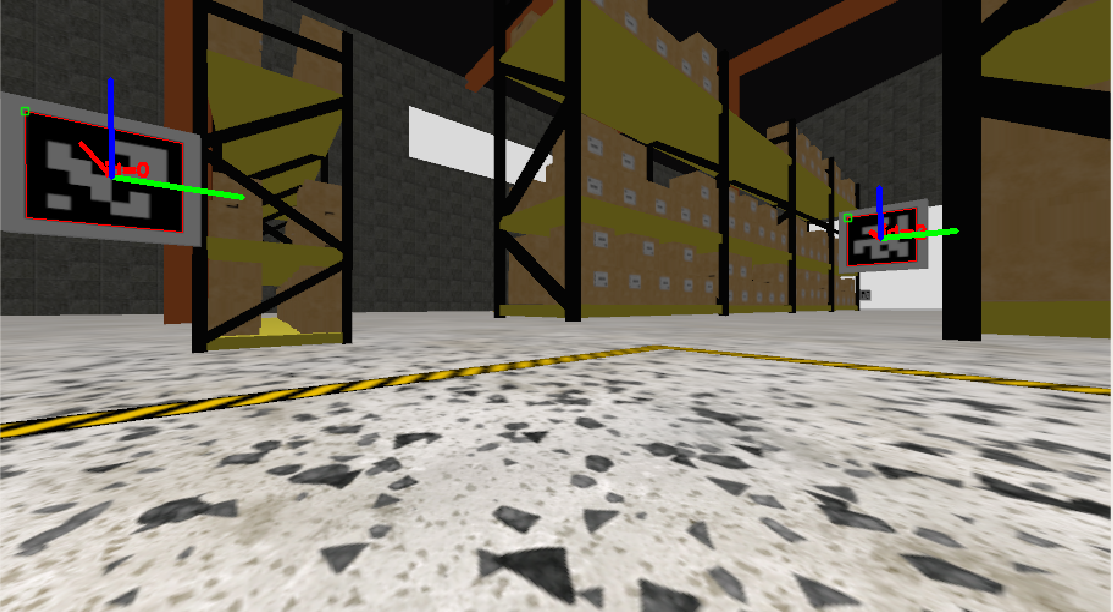
\includegraphics[width=0.9\linewidth]{img/cv_aruco}
				\caption[Carrolac]{Identificación y estimación de la pose de los marcadores}
				\label{fig:cv_aruco}
			\end{figure}

			Al conocer la pose real del marcador, se puede hacer una corrección de la pose de la base móvil estimada por la odometría para hacer que coincida la pose real con la pose observada del marcador por el robot.
			En la Figura~\ref{fig:cv_errores} se muestran los errores relativos entra la pose real de cada marcador y la estimada por el robot en Rviz.
			Los errores se visualizan con una barra verde y representa el vector error de traslación entre el marcador real y el marcador estimado.
			El error de rotación también se tiene en cuenta en el algoritmo de localización pero no se muestra en esta figura.
			\begin{figure}[H]
				\centering
				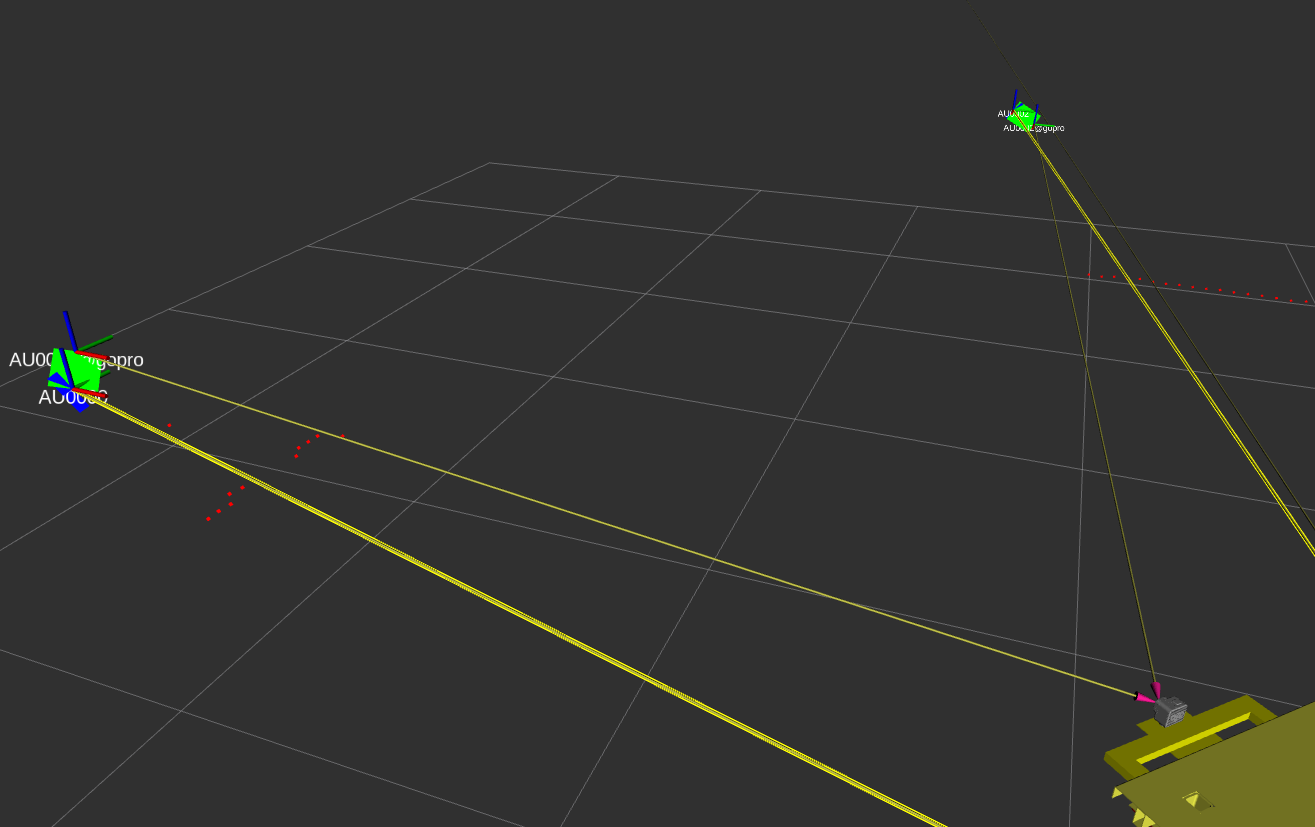
\includegraphics[width=0.9\linewidth]{img/cv_errores}
				\caption{Error de traslación de los marcadores}
				\label{fig:cv_errores}
			\end{figure}

			\section{Árbol de Sistemas de Referencia}\label{sec:algoritmo-localizacion/arbol-sist-ref}
				Es importante explicitar slos sistemas de referencia utilizados en el algoritmo y su interdependencia.
				A continuación se muestra un extracto del árbol de sistemas de referencia utilizado.
				\begin{Verbatim}[baselinestretch=0.1,label={verb:tftree}]

map   # S.REF FIJO AL MUNDO
|- AU0000   # S.REF DEL ARUCO CON ID=0 RESPECTO A 'map'
|- ...
|- AUwxyz   # S.REF DEL ARUCO CON ID=wxyz RESPECTO A 'map'
|- odom:    # S.REF DE LA ODOMETRIA RESPECTO A 'map'
   |- link_base  # S.REF DE LA BASE RESPECTO A 'odom'
      |- ...
         |- ...
            |- camera_optical # PLANO OPTICO DE LA CAMARA
               |- AU0000@camera # S.REF DEL ARUCO CON ID=0 RELATIVO
               |- ...
               |- AUwxyz@camera # S.REF DEL ARUCO CON ID=wxyz RELATIVO
				\end{Verbatim}
				Los nombres de algunos sistemas de referencia mostrados no coinciden necesariamente con el nombre exacto implementado para facilitar la interpretación conceptual.
				\begin{itemize}
					\item \texttt{map}: Sistema de referencia fijo al mundo.
					Representa el origen del sistema de coordenadas del entorno.
					\item \texttt{AU****}: Estos sistemas de coordenadas representan la pose de los marcadores ArUco respecto al mapa.
					Es decir, representan la pose \("\)real\("\) (o de Gazebo) de los marcadores
					\item \texttt{odom}: Es el origen del sistema de referencia de la odometría.
					Idealmente, coincidiría con \texttt{map}, pero como la odometría acumula errores se debe corregir.
					La diferencia entre \texttt{map} y \texttt{odom} representa la corrección de localización por el algoritmo implementado.
					\item \texttt{link\_base}: Sistema de referencia de la base móvil.
					La posición relativa entre \texttt{odom} y \texttt{link\_base} está dada por el cómputo de la odometría de la base móvil y debe dibujar una trayectoria suave y continua en el tiempo
					\item \texttt{camera\_optical}: representa la posición del plano óptico de la cámara respecto a la base móvil
					\item \texttt{AU****@camera}: representa el sistema de referencia de los marcadores ArUco estimados relativos a la cámara.
				\end{itemize}

				Para lograr el objetivo, el algoritmo de localización por computadora debe hacer coincidir la pose global (respecto a \texttt{map}) de los sistemas de referencia \texttt{AU****} con la de su homólogo asociado \texttt{AU****@camera} mediante la modificación de la pose de \texttt{odom} respecto a \texttt{map}.

				En este trabajo en particular, como se utilizó un modelo de cámara tipo GoPro, en la implementación se encontrará el identificador \texttt{gopro} en lugar del identificador \texttt{camera} donde corresponda.
			\section{Implementación}\label{sec:algoritmo-localizacion/implementacion}
				El algoritmo fue implementado en un nodo de ROS2 en Python en el archivo \texttt{src/computer\_vision/computer\_vision/aruco\_detector.py} del repositorio.
				El nodo se subscribe a los tópicos de la imagen de la cámara y, al recibir un nuevo mensaje de imagen llama a la función \texttt{image\_callback()}.
				Esta función utiliza la función \texttt{detectMarkers(img)} de la clase\linebreak\texttt{cv2.aruco.ArucoDetector} para detectar los marcadores en la imagen.
				Esta función devuelve las esquinas y los identificadores de los marcadores encontrados, que posteriormente son dibujados con\linebreak\texttt{cv2.aruco.drawDetectedMarkers(...)}.
				Para cada marcador, va a calcular la pose relativa a la cámara con \texttt{cv2.solvePnP(...)}.
				Con estos datos, dibuja el sistema de referencia del marcador en la imagen de la cámara, publica esta nueva imagen en otro tópico y también publica en ROS la transformación \texttt{AU****@camera} entre el marcador y la cámara.

				Por otra parte, un temporizador llama constantemente a la función\linebreak\texttt{on\_tf\_timer()} en donde evalúa si hay transformaciones del tipo \linebreak\texttt{AU****@camera} publicadas en ROS\@.
				En caso que las hubiera, determina el error tanto en traslación como en rotación entre \texttt{AU****} y \texttt{AU****@camera} a través de la función \texttt{lookup\_transform()} de la clase \texttt{tf2\_ros.Buffer}.
				Luego, los vectores error son trasladados al sistema de referencia del mapa para formar un error promedio de traslación y un error promedio de rotación entre todos los marcadores detectados en ese momento.
				Con los vectores errores, se modifica dinámicamente el sistema de referencia \texttt{odom} utilizando un filtro proporcional Kp.
				Se destaca que para reducir el error de orientación, se trabaja con vector de rotación y no con matriz de rotación o cuaternión.
				Esto es porque el vector de rotación  permite sumar o restar las componentes y mantener una rotación suave y continua.
				El vector de rotación es un vector de 3 componentes en donde el versor asociado representa la dirección sobra la que se efectúa la rotación y la magnitud del vector es la magnitud del ángulo girado.

			\section{ArUcos en Gazebo}
				Los marcadores ArUco fueron modelados en Blender y colocados en posiciones conocidas en el mundo de Gazebo.
				Cada marcador tiene un identificador ($i$) de marcador ArUco al frente y en su lado de opuesto tiene identificador ($i+1$). Por ejemplo, el marcador \texttt{AU0000} con pose $[x_0, y_0, z_0, r_x_0, r_y_0, r_z_0]$ tiene la misma posición que el \texttt{AU0001} pero rotado $180^{\circ}$ en su eje $z$ local.

%				El código detallado y completo de este nodo se muestra en el Apéndice~\ref{sec:aruco_detector.py}

	\chapter{Resultados}\label{ch:resultados}
		El video indicado en la Sección~\ref{sec:repositorios} muestra la visualización en Rviz de los resultados obtenidos.
		En el video mostrado, el robot comienza en el origen, es decir, los sistemas de referencia \texttt{map}, \texttt{odom} y \texttt{link\_base} coinciden al comienzo de la simulación.
		Esta situación se muestra en la Figura~\ref{fig:resultados-condicion_inicial}.

		\begin{figure}[H]
			\centering
			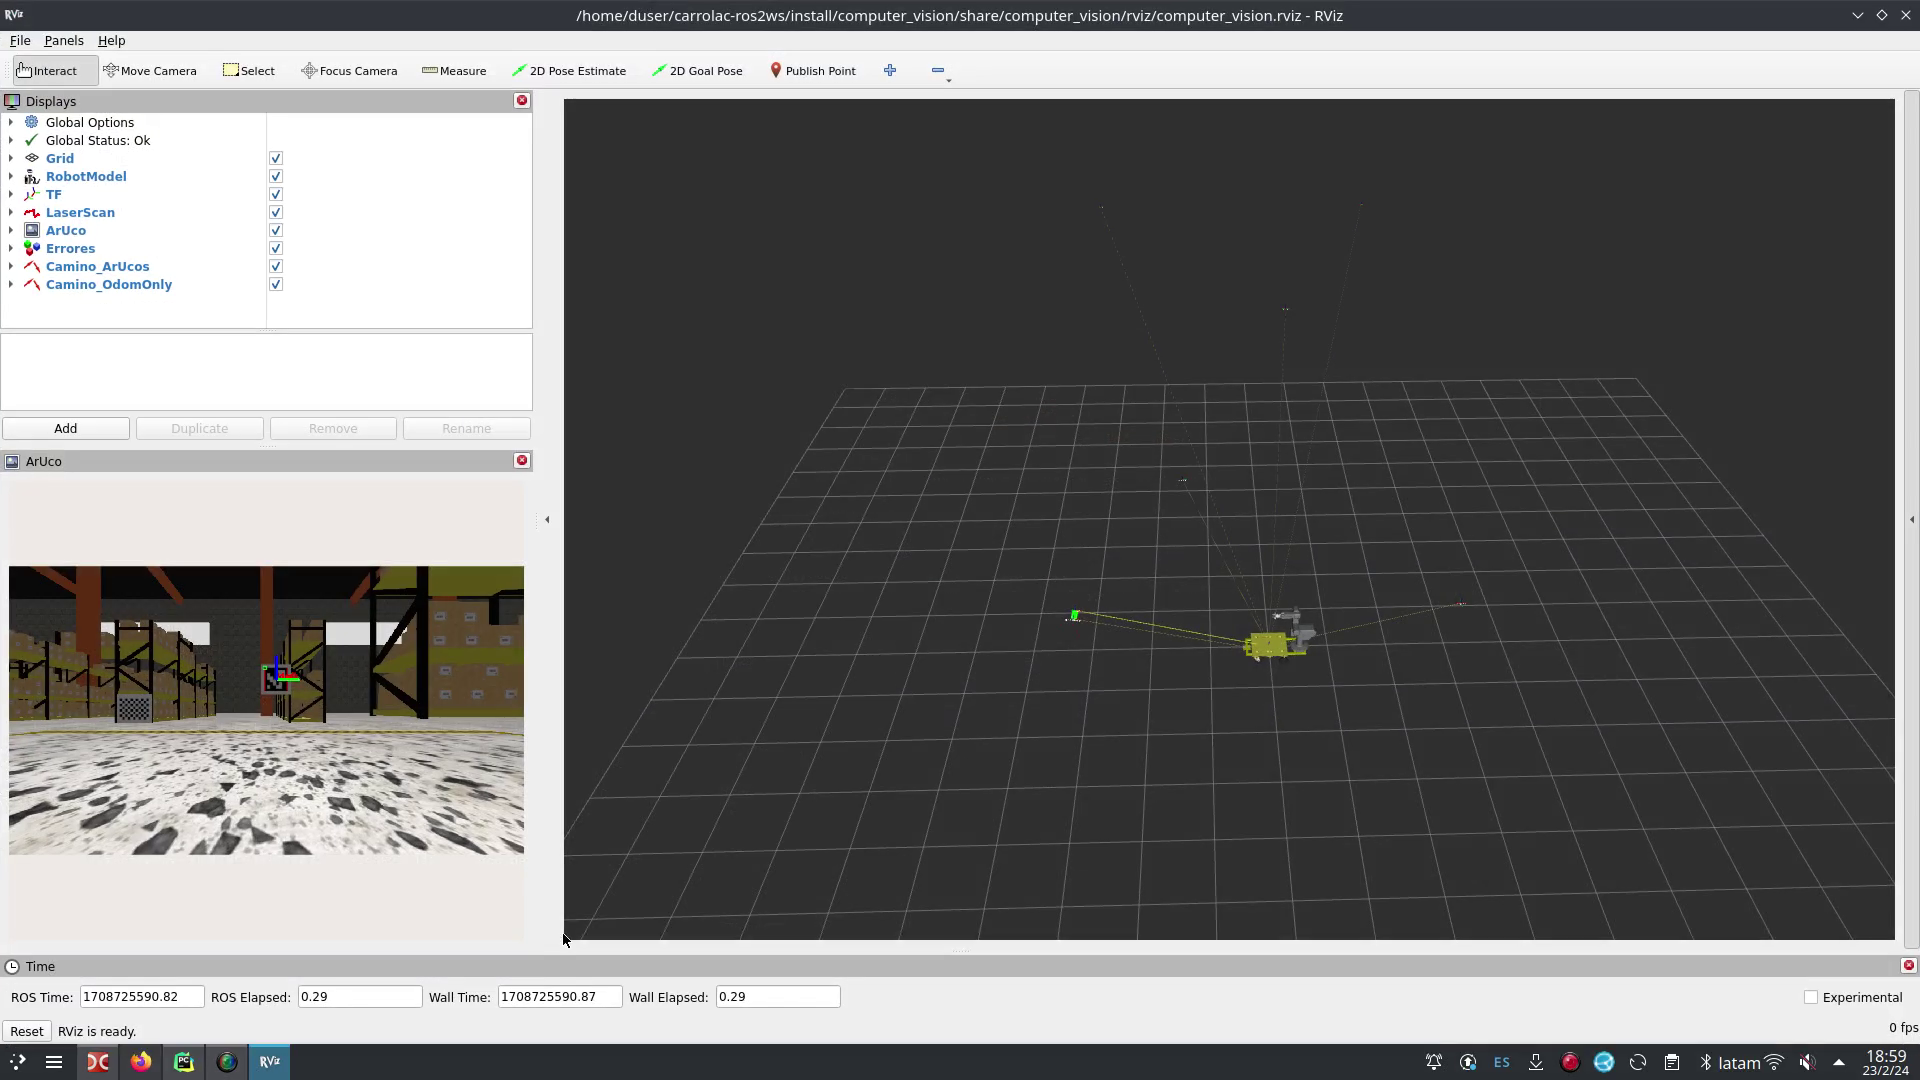
\includegraphics[width=1\linewidth]{img/vlcsnap-2024-02-28-10h36m58s557}
			\caption{Resultados en Rviz. Condición Inicial}
			\label{fig:resultados-condicion_inicial}
		\end{figure}

		A medida que el carro se mueve se computa la odometría y el sistema \texttt{link\_base} comienza a moverse continuamente respecto a \texttt{odom}.

		Cuando la cámara del robot capta un marcador aruco, el sistema de referencia local del marcador es dibujado en la propia imagen de la cámara y también se agrega a la visualización 3D con el nombre \texttt{AU****@gopro}.
		Al darse esta situación se agrega, entre los sistemas de referencias del marcardor detectado y el original, una barra verde representado el error de traslación y una azul representa el error de rotación como vector como se muestra en la Figura~\ref{fig:resultados-errores_locales}

		\begin{figure}[H]
			\centering
			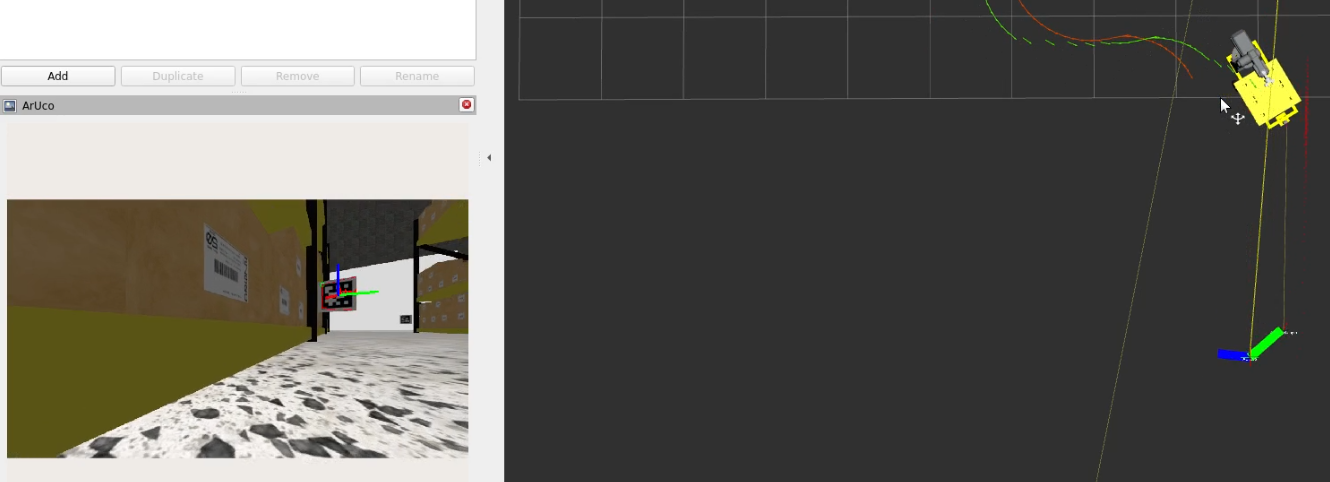
\includegraphics[width=1\linewidth]{img/Captura desde 2024-02-28 11-03-31}
			\caption{Error de traslación (verde) y rotación (azul) locales a un marcador}
			\label{fig:resultados-errores_locales}
		\end{figure}

		Los errores de traslación y rotación locales a cada marcador son trasladados instantáneamente al origen del mapa (\texttt{map}).
		En \texttt{map} queda finalmente un error de traslación total, en rojo, que representa el promedio de todos los errores de traslación detectados en ese instante; y un error de rotación total, en cian, que representa el promedio de todos los errores de rotación detectados en ese instante.
		Esta situación se muestra en la Figura~\ref{fig:resultados-errores_map}.
		\begin{figure}[H]
			\centering
			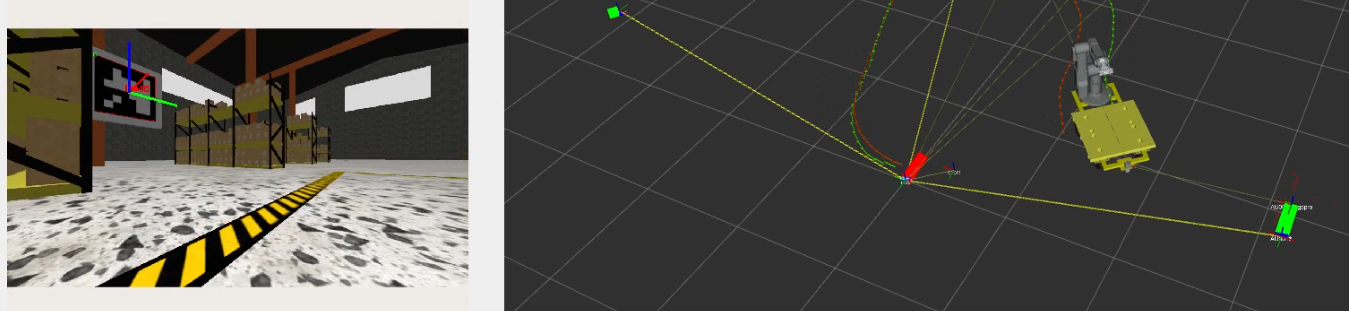
\includegraphics[width=1\linewidth]{img/Captura desde 2024-02-28 10-47-31}
			\caption{Errores trasladados al origen del mapa (\texttt{map}).}
			\label{fig:resultados-errores_map}
		\end{figure}

		En este sentido, el sistema \texttt{odom} va a trasladarse y rotar respecto a \texttt{map} con una velocidad proporcional a los vectores error de traslación y rotación, respectivamente.
		De esta forma, el sistema \texttt{odom} se va a mover suavemente de manera que los sistemas instantáneos \texttt{AU****@gopro} converjan en posición y orientación a los \texttt{AU****}.
		Como ya se explicó, esta converjencia se hace desplazando el sistema \texttt{odom}.
		En la Figura~\ref{fig:resultados-convergencia} se muestra la corrección del camino en el sistema fijo \texttt{map}.
		Se puede ver la convergencia asintótica a una pose que hace coincidir los sistemas del marcador ArUco.
		Cuánto más grande el error, mayor es la velocidad con la que se reduce el error.

		\begin{figure}[H]
			\centering
			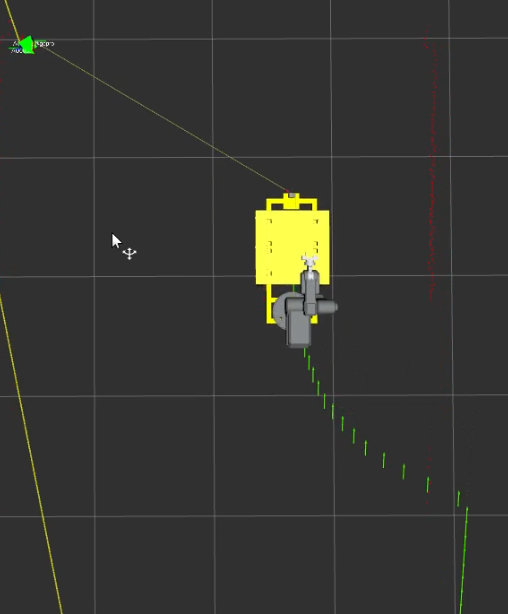
\includegraphics[width=1\linewidth]{img/Captura desde 2024-02-28 11-05-30}
			\caption{Convergencia del camino corregido (verde).}
			\label{fig:resultados-convergencia}
		\end{figure}

		Finalmente, en la Figura~\ref{fig:resultados-comparacion} se muestran comparativamente el camino sin corrección (en naranja), es decir, utilizando únicamente la odometría, y el camino corregido con los marcadores ArUco (en verde).

		\begin{figure}[H]
			\centering
			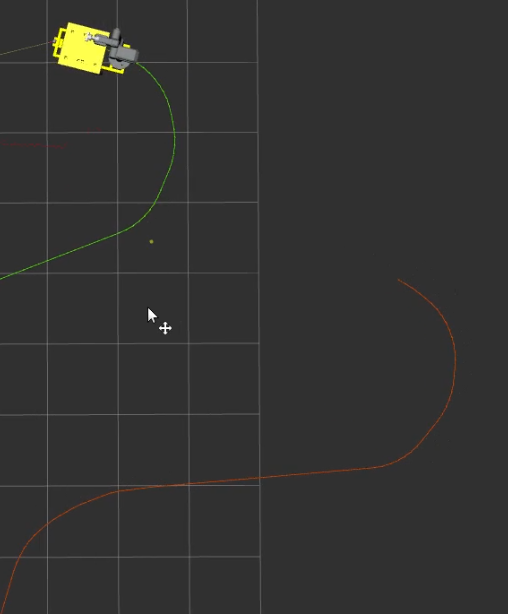
\includegraphics[width=1\linewidth]{img/Captura desde 2024-02-28 11-11-17}
			\caption{Comparación con (verde)/sin (naranja) detección de ArUco}
			\label{fig:resultados-comparacion}
		\end{figure}

	\chapter{Guía de uso}\label{ch:guia-de-uso}
		En este capítulo se provee una guía de uso para replicar los resultados obtenidos y/o ejecutar nuevos ensayos y modificaciones en los algoritmos.

		\section{Estructura del repositorio}\label{sec:estructura-del-repositorio}
	En primer lugar, se debe clonar en la computadora local el repositorio de Git mencionado en la Sección~\ref{sec:repositorios}:
			\begin{lstlisting}[language=Bash,label={lst:lstlisting}]
$ git clone git@github.com:guillerolle/carrolac-project.git
			\end{lstlisting}
			En el directorio base se encuentran las siguientes carpetas:
			\begin{itemize}
				\item \texttt{carrolac-ros2ws}: Es el workspace de ROS y Gazebo del proyecto.
					Dentro del mismo, contiene la carpeta \texttt{src} con todos los archivos fuente de los paquetes implementados en este proyecto.
				\item \texttt{docker-home}: Este directorio se usa como punto de montaje para \texttt{\$HOME} del contenedor Docker.
				\item \texttt{docker-sources}: Contiene puntos de montaje de distintos archivos fuente de ROS que están incluidos en la imagen de Docker.
					Permite tener referencias a clases y funciones de los paquetes instalados de ROS desde un IDE externo al Docker.
				\item \texttt{informe}: Archivos fuente del informe
				\item \texttt{scripts}: Scripts de asistencia para ejecución rápida y automática de ciertas funcionalidades.
				\item \texttt{venvs}: En este directorio se dispondrán los entornos virtuales de Python que se utilizan tanto en el IDE externo al Docker para programar los nodos, como el interno a Docker desde donde cargará los paquetes específicos de Python para la ejecución propiamente de los nodos.
			\end{itemize}

		\section{Guía de uso del Docker}\label{sec:guia-de-uso-del-docker}
	El símbolo * en los nombres de las siguientes subsecciones significa que son pasos que se deben ejecutar una única vez para poner en funcionamiento el entorno.
			No es necesario ejecutarlas cada vez que quiera correr algún nodo.
			Todos los scripts deben ser ejecutados desde la carpeta \texttt{scripts} para que funcionen correctamente.
			\subsection{Compilación del Docker*}\label{subsec:compilacion-del-docker*}
	Primero se debe compilar la imagen del docker se debe correr el script auxiliar \texttt{compile\_docker.sh}.
			\subsection{Preparación del entorno virtual de Python*}\label{subsec:preparacion-del-entorno-virtual-de-python}
	Antes de poder ejecutar cualquier nodo, es necesario preparar el entorno de Python con las librerías necesarias en este proyecto.

				Al ejecutar el script \texttt{start\_docker\_graphics.sh}, se iniciar el contenedor con los puntos de montajes necesarios.
				Al iniciar docker, debería aparecer la leyenda \texttt{SOURCEANDO .BASHRC...} en la terminal, indicando que el \texttt{\$HOME} del Docker está correctamente montado.
				La primera vez que se ejecuta, debería mostrarse un error al hacer \texttt{source ~/.bashrc} porque no se encuentra el entorno virtual de Python.

				Dentro de la terminal del contenedor, debería haber una carpeta \texttt{~/venvs}, que es un punto de montaje de la carpeta \texttt{venvs} del repositorio.
				Para crear el entorno virtual, correr las siguientes líneas:
				\begin{lstlisting}[language=Bash, label={lst:create_venv}]
$ cd ~/venvs
$ ./create_venv.sh
				\end{lstlisting}
				El script \texttt{create\_venv.sh} crea un entorno virtual de Python en el directorio correspondiente para ser cargado automáticametne por \texttt{.bashrc} y con las librerías necesarias indicadas en \texttt{requirements.txt}.

			\subsection{Compilación del Workspace*}\label{subsec:compilacion-del-workspace*}
				Para compilar el Workspace de ROS, desde la máquina HOST se debe correr el script \texttt{build\_workspace.sh}.
				El workspace debería compilarse correctamente y los archivos de compilación deberían aparecer en la carpeta \texttt{carrolac-ros2ws} del HOST.

			\subsection{Inicio del Contendor}\label{subsec:inicio-del-contendor}
	Para iniciar el contenedor con todas las funcionalidades necesarias luego de ejecutar todos los pasos anteriores al menos una vez, basta con ejecutar el script \texttt{start\_docker\_graphics.sh}.
				Se iniciará una terminal dentro del contenedor y debería aparecer la leyenda \texttt{SOURCEANDO .BASHRC} sin ningún error ni mensajes a continuación.

			\subsection{Anexar otra terminal al contenedor}
				Para conectarse al contenedor con más de una terminal, una vez iniciado el contenedor como se indica en la subsección~\ref{subsec:inicio-del-contendor}, se debe ejecutar el script \texttt{connect\_docker.sh}.
		\section{Guía de ROS y Gazebo}
			\subsection{Ejecutar Simulación completa}
				Es posible que la primera vez que se ejecute la simulación en Gazebo, ésta tarde bastante para iniciar porque Gazebo debe descargar los modelos de la fábrica utilizados en el mundo.

				Para ejecutar el mundo de simulación en Gazebo, una vez iniciado un contenedor de Docker correctamente (sección~\ref{subsec:inicio-del-contendor}), se ejecuta el comando
				\begin{lstlisting}[language=Bash, label={lst:launch_gazebo}]
$ ros2 launch carrolac_gazebo gazebo.launch.py
				\end{lstlisting}
				El archivo launch mostrado acepta los siguientes parámetros:
				\begin{itemize}
					\item \texttt{sim\_on:=\{True|False\}}: Indica si la simulación de Gazebo inicia pausada (False) o corriendo (True)
					\item \texttt{bag\_on:=\{True|False\}}: Indica si se generará o no un bag de la simulación.
						Tener en cuenta que los bag files pueden ser del orden de decenas de GB si se guardan todos los nodos juntos.
					\item \texttt{computer\_vision:=\{True|False\}}: Indica si se ejecutará el nodo de computer vision.
						El algoritmo de localización puede funcionar en vivo durante la simulación o reproduciendo un rosbag.
					\item \texttt{rviz:=\{True|False\}}: Indica si inicia o no Rviz.
					 	Debería iniciarse solamente con \texttt{computer\_vision:=True}
					\item \texttt{rqt\_on:=\{True|False\}}: Inicia rqt con una visualización del árbol de TF y la imagen original de la cámara.
						Útil para debug de códigos.
				\end{itemize}
				Por ejemplo, las 2 ejecuciones más comunes de la simulación son:
				\begin{lstlisting}[language=Bash, label={lst:launch_gazebo_cvon}]
$ ros2 launch carrolac_gazebo gazebo.launch.py sim_on:=True bag_on:=False computer_vision:=True rviz:=True, rqt_on:=False
				\end{lstlisting}
				para correr el nodo de computer vision en vivo, o:
				\begin{lstlisting}[language=Bash, label={lst:launch_gazebo_cvoff}]
$ ros2 launch carrolac_gazebo gazebo.launch.py sim_on:=True bag_on:=True computer_vision:=False rviz:=False, rqt_on:=False
				\end{lstlisting}
				para guardar un bag file de la simulación, para luego probar el nodo de computer vision sin gastar recursos computacionales en la simulación.

				\subsubsection{Control de la plataforma móvil en Gazebo}
					Cualquiera sea la forma elegida para ejecutar la simulación, la base móvil se puede controlar manualmente con teclado con las teclas \texttt{WASD}:
					\begin{itemize}
						\item \texttt{W}: mueve la base móvil hacia adelante
						\item \texttt{S}: mueve la base móvil hacia atrás
						\item \texttt{A}: rota la base móvil en sentido antihorario
						\item \texttt{D}: rota la base móvil en sentido horario
					\end{itemize}

			\subsection{Rosbag con Computer-Vision}
				La otra opción, más eficiente para probar el nodo implementado de computer vision es: lanzar un rosbag con los datos de la simulación propiamente dicha y luego lanzar, encima, el nodo de correción con los ArUco.
				Se incorporó un archivo launch que gestiona esta situación.
				Para esto es necesario descargar el rosbag del Mega indicado en la sección~\ref{sec:repositorios} y descomprimirlo en la carpeta \texttt{carrolac-ros2ws/bags}.
				Una vez hecho esto, se puede ejecutar:
				\begin{lstlisting}[language=Bash, label={lst:launch_rosbagcv}]
$ ros2 launch computer\_vision aruco.launch.py bag_on:=True bag_file:=bags/2024_02_23-18_43_03
				\end{lstlisting}
				donde, los argumentos son:
				\begin{itemize}
					\item \texttt{bag\_on:=\{True|False\}}: Activa o desactiva la carga automática de un rosbag
					\item \texttt{bag\_file:=<string>}: Si \texttt{bag\_on:=True}, indica cuál es el rosbag a cargar
				\end{itemize}

%			\pendiente[inline]{Agregar calibración de la cámara}

		\subsection{Calibración de la Cámara}
			Aunque la cámara es simulada en Gazebo, es necesario identificar los parámetros intrínsecos de la misma.
			Para esto, en el mismo mundo de Gazebo se incorporó un cartón calibrador tipo checkerboard como se muestra en la Figura~\ref{fig:calibracion-checkerboard}

		\begin{figure}[H]
			\centering
			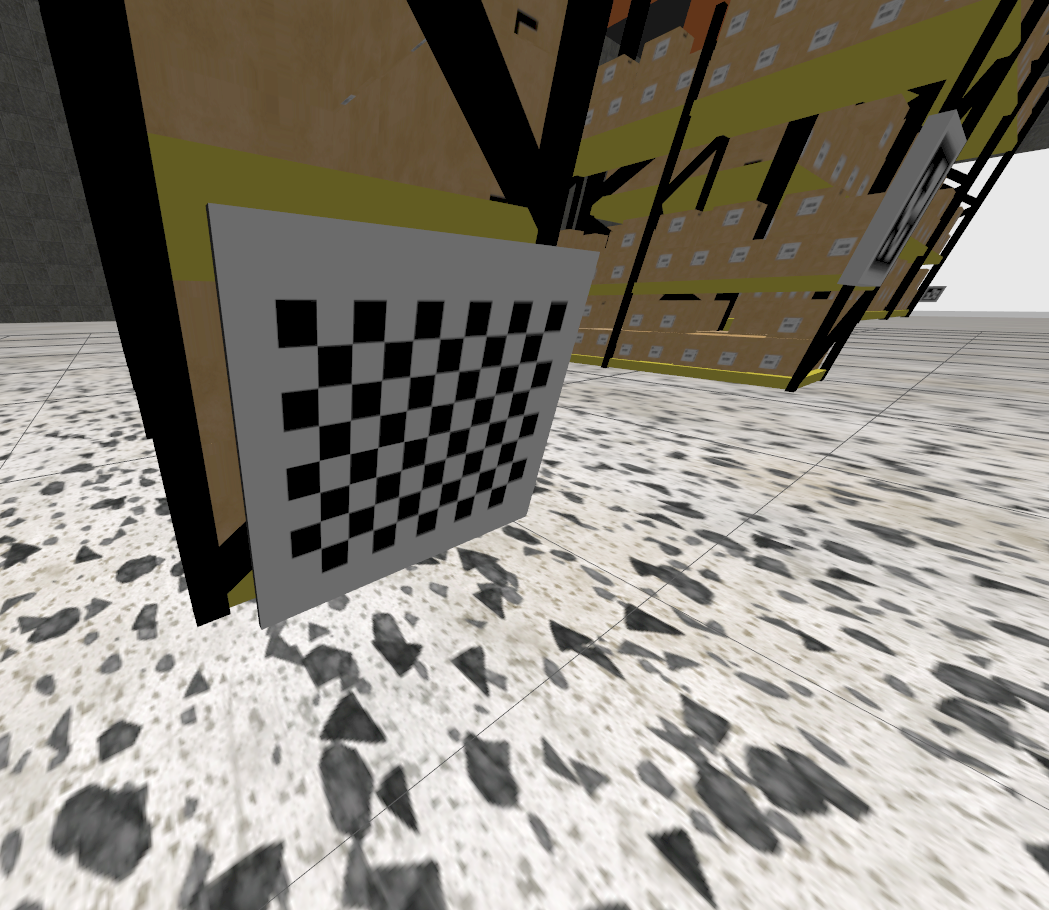
\includegraphics[width=0.7\linewidth]{img/Screenshot_20240228_143927}
			\caption{Checkerboard para calibración de la cámara}
			\label{fig:calibracion-checkerboard}
		\end{figure}

			Para calibrar, es entonces necesario mover la base móvil y enfrentarla al checkerboard.
			Luego, se puede correr el siguiente nodo en otra terminal (usando el script \texttt{connect\_docker.sh}):
	\begin{lstlisting}[language=Bash,label={lst:lstlisting2}]
$ ros2 run camera_calibration cameracalibrator --camera_name gopro --pattern chessboard --size 7x10 --square 0.015 --no-service-check --ros-args -r image:=/gopro_camera/image_raw --log-level DEBUG
	\end{lstlisting}

		\begin{figure}[H]
			\centering
			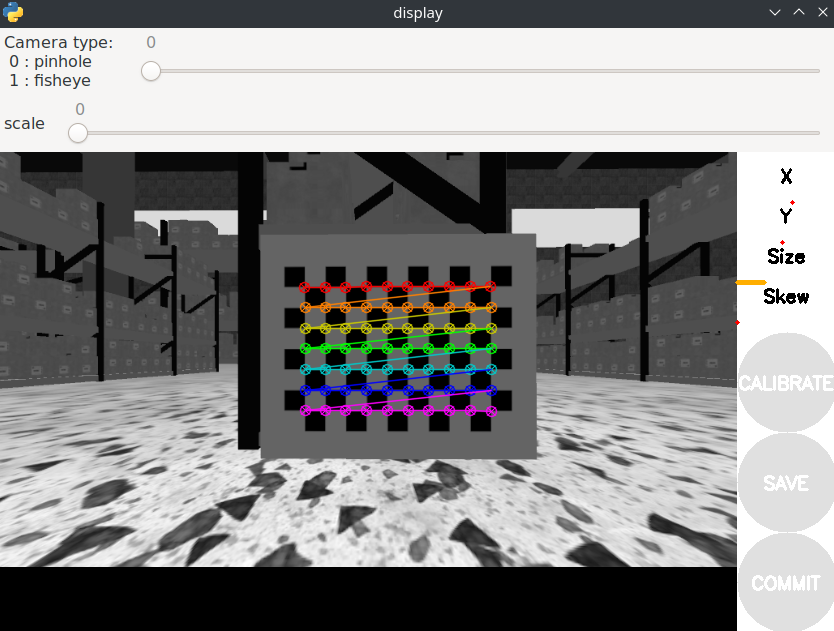
\includegraphics[width=0.7\linewidth]{img/Screenshot_20240228_144839}
			\caption{Calibrador de la cámara}
			\label{fig:calibracion-calibrator}
		\end{figure}

			Una vez abierto el calibrador y detectado el patrón, se puede ejecutar el siguiente script para producir movimientos en el checkerboard y facilitar la calibración de la cámara:
	\begin{lstlisting}[language=Bash,label={lst:lstlisting3}]
$ cd ~/carrolac-ros2ws/src/computer_vision/camera_calibrator
$ ./move_calibrator_checkerboard.py
	\end{lstlisting}

	\begin{figure}[H]
		\centering
		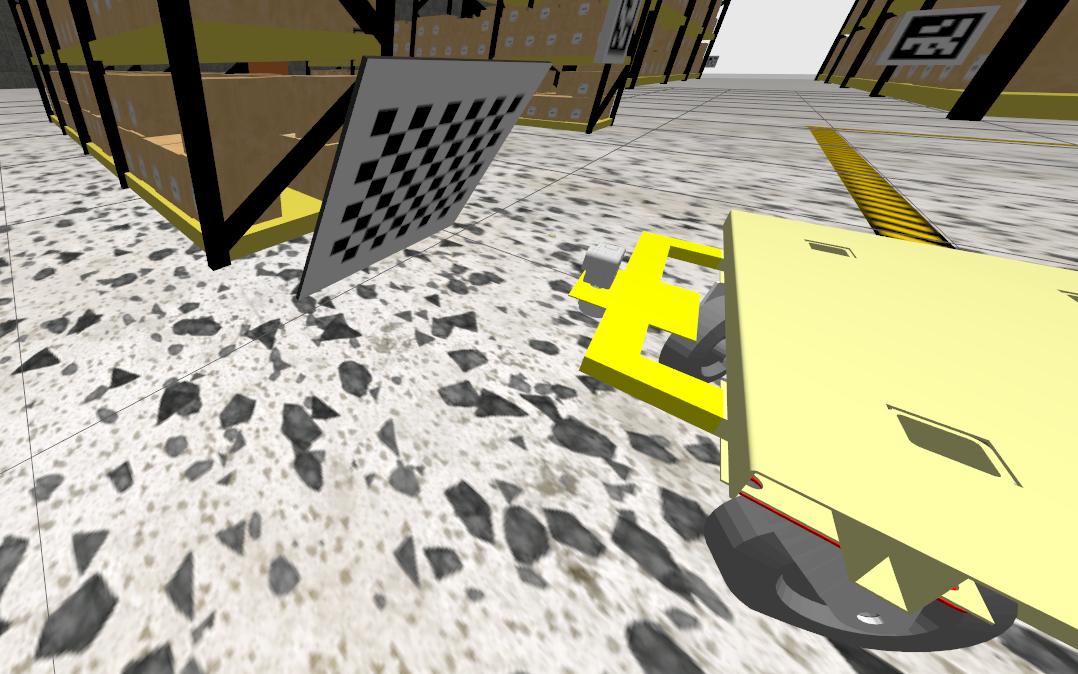
\includegraphics[width=0.7\linewidth]{img/Screenshot_20240228_145154}
		\caption{Checkerboard inclinado durante calibración}
		\label{fig:calibracion-cb-inclinado}
	\end{figure}

	La calibración arrojará los parámetros intrínsicos y distorsión de la cámara, parámetros que son necesarios para detectar correctamente la pose relativa a los marcadores ArUco.

	\subsubsection{Comentario sobre la implementación}
	Si bien se pudo calibrar correctamente la cámara, no fue posible incorporar los datos de la calibración en Gazebo.
	Esto significa que, aunque se pueda modificar la resolución, campo de visión y más parámetros dentro de los mismos URDF y esto es correctamente leído por Gazebo, no se encontró forma de hacer que Gazebo publique correctamente los parámetros en el tópico \texttt{image\_info}, ya que siempre publica los mismos valores por defectos sin importar los cambios que se hagan en el URDF.
	Debido a esto, los parámetros de la cámara son hardcodeados en la implementación del nodo en Python directamente.
	Lógicamente, este método está lejos de ser ideal pero no hubo éxito en implementarlo de una manera más correcta.

	\chapter{Conclusiones}
		En el presente trabajo se implementó un método de localización para ambientes interiores de una base móvil utilizando marcadores ArUco y visión por computadora, aplicado particularmente a un modelo de simulación que es pertinente al grupo del Laboratorio.
		El prototipo de manipulador móvil usado fue desarrollado exclusivamente para este fin, aunque se prevé su uso para muchos otros estudios de interés para el grupo.

		El diseño en formato \texttt{urdf} fue pensado de forma modular, de forma que se puedan crear varias bases/manipuladores móviles de diferentes características incluyendo módulos específicos en cada caso.
		El formato modular de los \texttt{urdf} no fue probado exhaustivamente para este trabajo pero sirve para tener una primera versión de archivos.

		Los algoritmos de visión por computadora fueron probados en Gazebo y se verificó un funcionamiento aceptable en general, aunque aparecieron muchas aristas para evidentes mejoras.
		Por ejemplo, al vibrar la cámara cuando se desplaza el robot se introduce mucho ruido en la imagen y esto se traslada a errores grandes en el posicionamiento, incluso llevando a la divergencia en algunos casos (raros), debido también al método de combinación de sensores (usando un filtro Proporcional).
		Otra problemática encontrada, es que este método requiere el conocimiento de la pose exacta de todos los marcadores ArUco en la fábrica.
		En la simulación eso no es problema, pero puede ser un problema al intentar implementarlo en la vida real.

		Como trabajo a futuro en relación a los contenidos dados en la materia, es de interés incorporarle al robot la generación de un mapa del entorno y verificarlo con planos reales.
		Esto podría ayudar al robot a navegar por la fábrica, verificando su posición real mediante los ArUcos colocados estratégicamente.


%	\begin{appendices}
%		\renewcommand{\chaptername}{Apéndice}
%
%		\chapter{Python Files}\label{app:python-files}
%		\section{aruco\_detector.py}\label{sec:aruco_detector.py}
%		\lstinputlisting[language=Python,label={lst:lstinputlisting22}]{../carrolac-ros2ws/src/computer_vision/computer_vision/aruco_detector.py}
%	\end{appendices}

\end{document}
